\documentclass[serif,mathserif]{beamer}


\usepackage{fleqn}
\usepackage{modefs}
\usepackage{math}
\usepackage[utf8]{inputenc}
\usepackage{amsmath, amsfonts, epsfig, xspace}
\usepackage{pstricks,pst-node}
\usepackage{multimedia}
\usepackage[normal,tight,center]{subfigure}
\usepackage{listings}
\setlength{\subfigcapskip}{-.5em}
\usepackage{beamerthemesplit}
\renewcommand\sfdefault{phv}
\renewcommand\familydefault{\sfdefault}
\usetheme{default}
\usepackage{color}
\useoutertheme{default}
\usepackage{texnansi}
\usepackage{marvosym}
\definecolor{bottomcolour}{rgb}{0.32,0.3,0.38}
\definecolor{middlecolour}{rgb}{0.08,0.08,0.16}
\setbeamerfont{title}{size=\Huge}
\setbeamercolor{structure}{fg=gray}
\setbeamertemplate{frametitle}[default]%[center]
\setbeamercolor{normal text}{bg=black, fg=white}
\setbeamertemplate{background canvas}[vertical shading]
[bottom=bottomcolour, middle=middlecolour, top=black]
\setbeamertemplate{items}[circle]
\setbeamerfont{frametitle}{size=\huge}
\setbeamertemplate{navigation symbols}{} %no nav symbols

\author[Vinicius Miana]{Vinicius Miana}

\title[Short Title\hspace{2em}\insertframenumber/\inserttotalframenumber]{Tutorial Mapkit e Localização}

\date{31 de janeiro de 2014} %leave out for today's date to be insterted

\institute{Universidade Presbiteriana Mackenzie}

\begin{document}

\maketitle

\section{Mapkit}  


\begin{frame}
  \frametitle{Crie o Projeto}
  \begin{figure}[t]
    \centering
    \subfigure[Escolha: New Project -> iOS -> Single View Application]{
      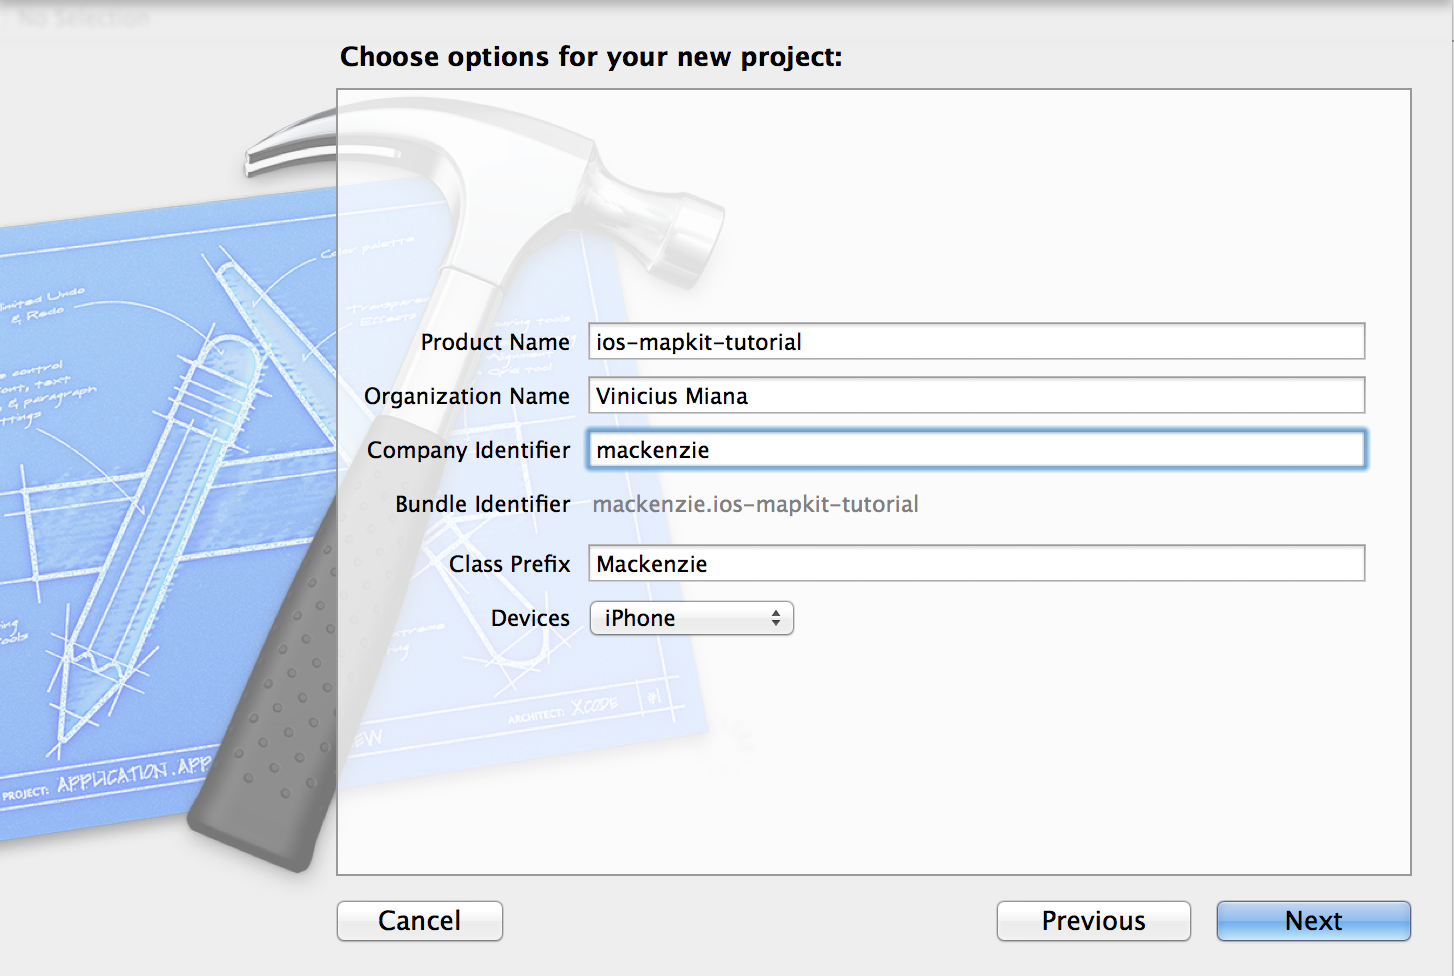
\includegraphics[width=10cm]{img/createProject.png}
    }
  \end{figure}
\end{frame}

\begin{frame}
  \frametitle{Adicione a Biblioteca Core Location}
  \begin{figure}[t]
    \centering
    \subfigure[Procure a seção Link Libraries e clique no +]{
      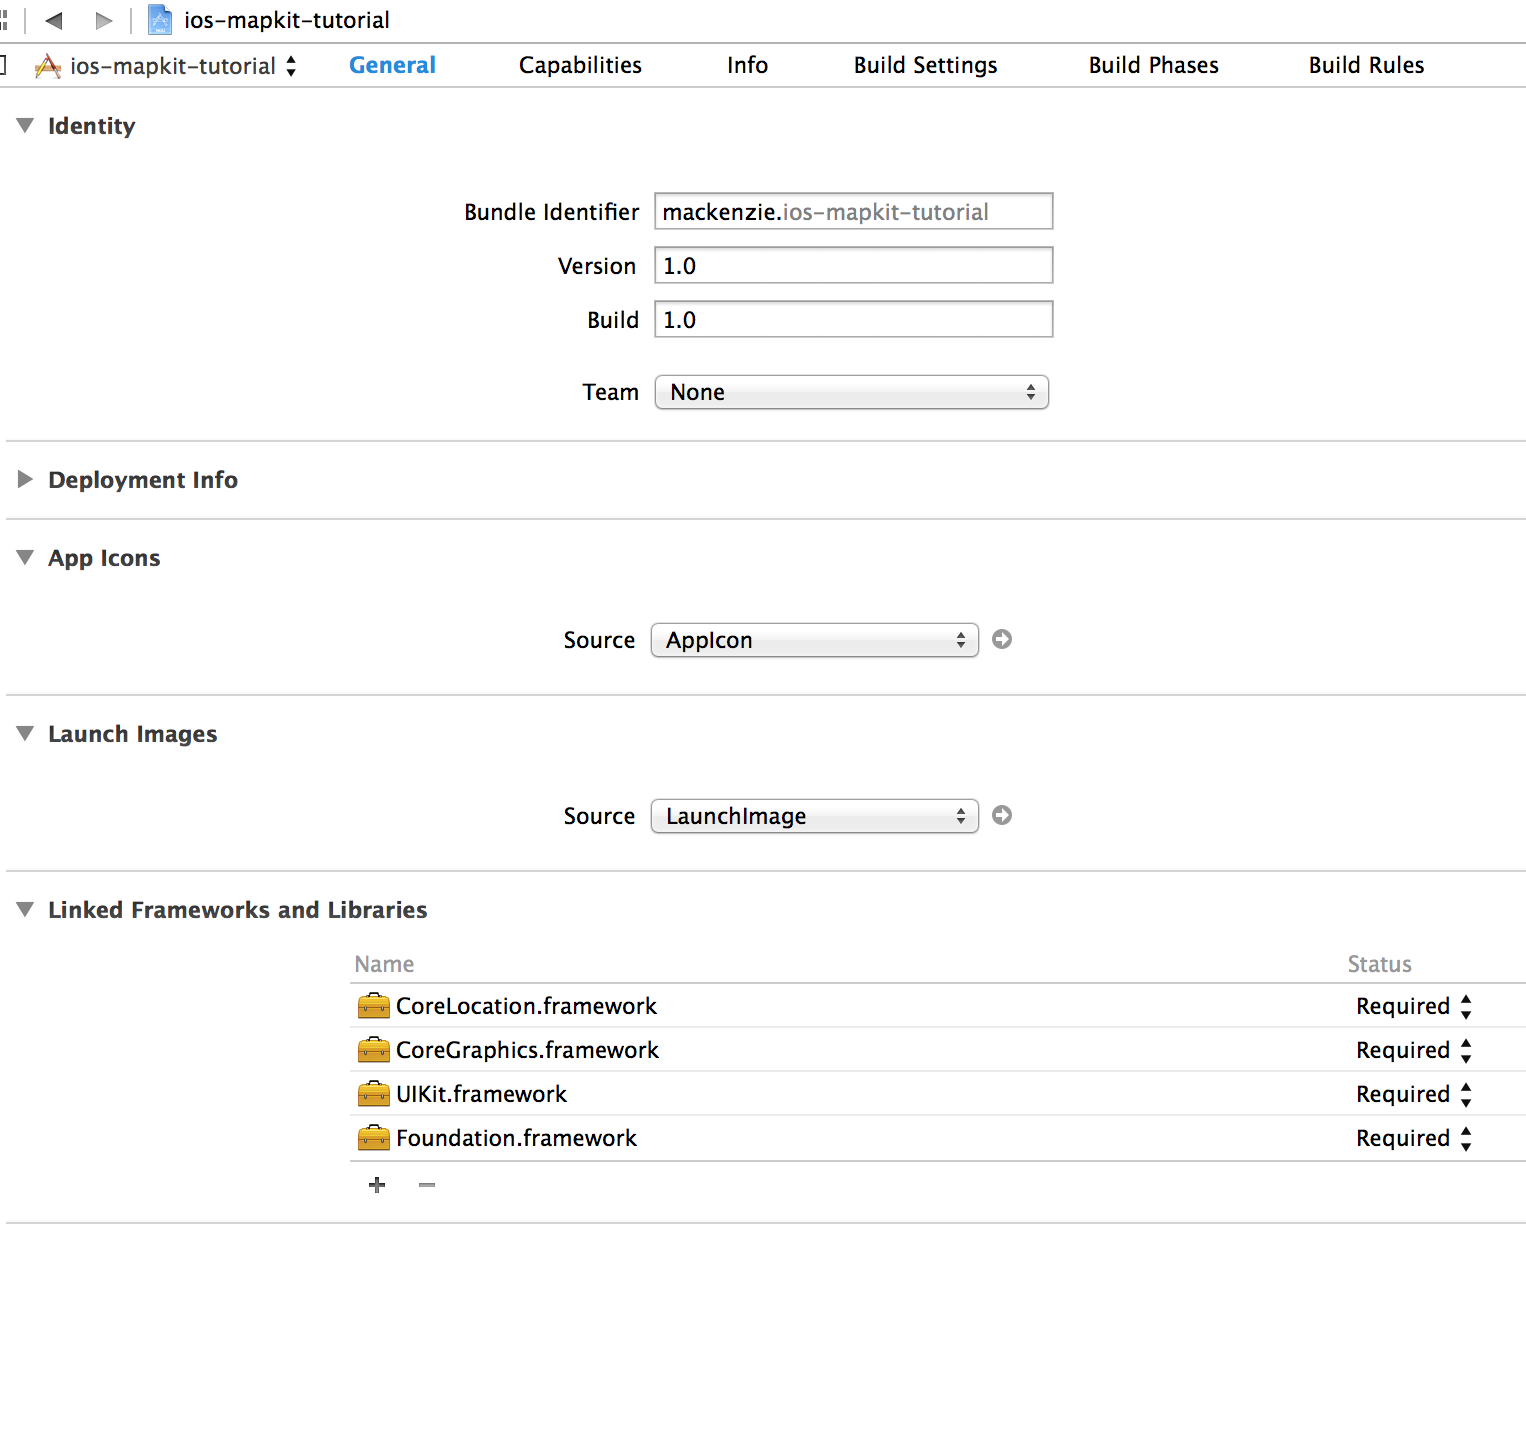
\includegraphics[width=5cm]{img/addLibrary.png}
    }
    \subfigure[Filtre para encontrar o CoreLocation e adicione]{
       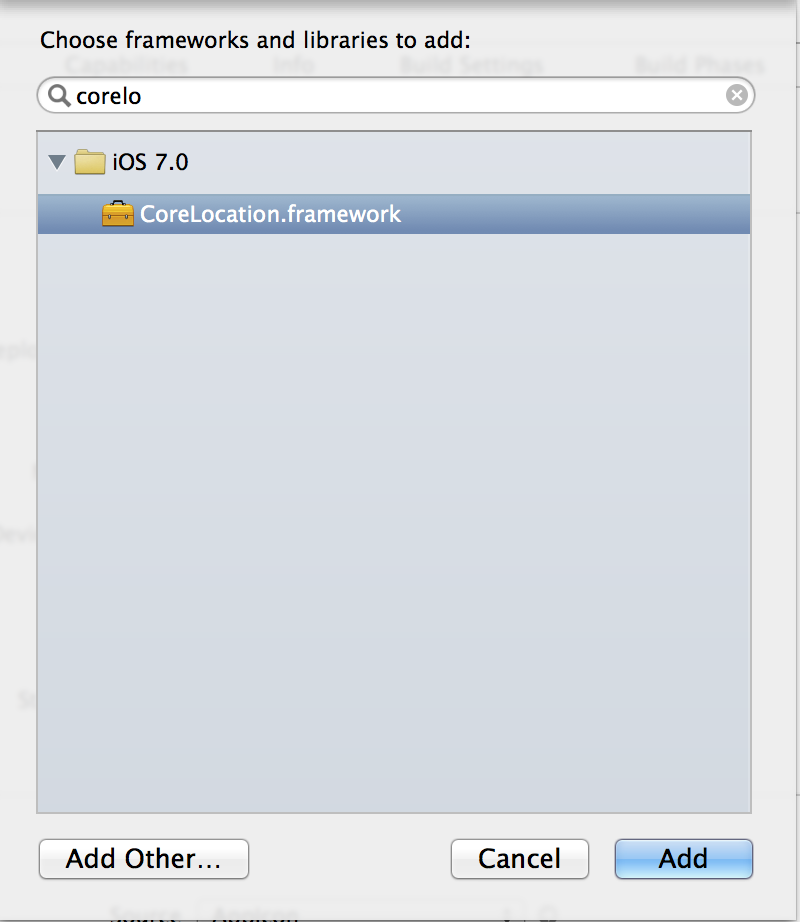
\includegraphics[width=5cm]{img/addLibrary2.png}
    }
  \end{figure}
\end{frame}


\begin{frame}[fragile]
  \frametitle{Adicione um CLLocationManager ao View Controler}
  ViewControler.h
  \lstset{language=[Objective]C, breakindent=40pt, breaklines}
  \begin{lstlisting}
    #import <UIKit/UIKit.h>
    #import <CoreLocation/CoreLocation.h>

    @interface MackenzieViewController :
                UIViewController<CLLocationManagerDelegate>
    {
      __weak IBOutlet MKMapView *mapView;
      CLLocationManager *locMgr;
    }
    @end
  \end{lstlisting}
\end{frame}


\begin{frame}[fragile]
  \frametitle{Inicialize o CLLocationManager}
  ViewControler.m
  \lstset{language=[Objective]C, breakindent=40pt, breaklines}
  \begin{lstlisting}
    -(id)initWithCoder:(NSCoder *)aDecoder {
      self = [super initWithCoder:aDecoder];
      if(self) {
        locMgr = [[CLLocationManager alloc] init];
        [locMgr setDelegate:self];
        [locMgr startUpdatingLocation];
      }
      return self;
    }
  \end{lstlisting}
\end{frame}


\begin{frame}[fragile]
  \frametitle{Implemente os métodos do CLLocationManagerDelegate}
  ViewControler.m
  \lstset{language=[Objective]C, breakindent=40pt, breaklines}
  \begin{lstlisting}
    -(void)locationManager:(CLLocationManager *)manager
                      didUpdateLocations:(NSArray *)locations {
      NSLog(@"Estou em %@",[locations lastObject]);
    }
    
    -(void)locationManager:(CLLocationManager *)manager
                       didFailWithError:(NSError *)error
    {
      NSLog(@"Erro %@",error);
    }

  \end{lstlisting}
\end{frame}





\begin{frame}
  \frametitle{Tarefas}
  Atividades:
  \begin{itemize}
  \item Pesquisar os métodos do CLLocationManager; 
  \item Alterar a frequencia de chamada do delegage;
  \item Centralizar o mapView na localizacao atual;
  \item Marcar pontos no mapa;
  \item Traçar o trajeto percorrido no mapa.
  \end{itemize}
\end{frame}





\begin{frame}
  \frametitle{Questions}
\end{frame}
\end{document}
